% vim: textwidth=78 ai spell spelllang=en filetype=tex sw=2

\section{Building Bug-database}\label{sec:clabure}
Necessity of a basis for improving static analyzers.

BSc thesis for web crawling (Ceľuch)

BSc thesis for web frontend (Hornák)

\stan output, SV-COMP~\cite{sv-comp} data

Implementing \cdb~\cite{claburedb}

\subsection{Introduction}\label{sec:introduction}

Many successful bug-finding tools based on various program analysis methods
appeared during the last ten years. None of them is perfect. Each tool
either reports both real errors and false positives, or it discovers only a
part of real errors. To improve or evaluate such a tool, one needs to run
the tool on some source codes and then analyze the obtained
bug-reports\footnote{We deliberately use term ``bug'' in the paper. It stems
from the need of the database to comprehend for example coding style
violations. In those cases, commonly used terms like ``failure'' or ``fault''
fail to apply.}, i.e.~classify them as false positives or real errors, and
find errors in the sources that were missed by the tool. This work is usually
tedious and time consuming, especially when one tunes or studies performance
of a tool for real software projects. The tedious work can be avoided if
suitable benchmarks, i.e.~programs with information about their errors, are
available.

There exist benchmark suites consisting of small synthetic
programs~\cite{CHK11,begbunch,KRA05,NCH05,srd} and those consisting of
real-world programs~\cite{begbunch,HW08,bugbench}. In benchmark
suites~\cite{CHK11,KRA05,NCH05}, relevant program locations in small
synthetic programs are explicitly marked as either erroneous or safe. The
benchmark suite~\cite{begbunch} marks only known real errors. The situation is
different for benchmarks with real-world programs: \cite{bugbench} contains
marked test cases triggering/non-triggering errors, while~\cite{HW08}
provides bug-reports (both real errors and false positives mixed together)
% without any differentiation)
produced by \textsc{Findbugs} and sorted
according to priority levels assigned to the reports by the tool. The
benchmark suites discussed so far consider different error types and provide
their own error taxonomies with exception of suites \cite{CHK11,begbunch},
where errors types are linked to \emph{Common Weakness Enumeration}
(\textsc{CWE})~\cite{cwe}.

As far as we know, there is no benchmark suite containing big real-life
projects with a significant list of uniformly described bug-reports
classified as real errors or false positives. Our benchmark suite \cdb
should fill this gap.

\cdb currently contains only a single project, namely the Linux kernel
2.6.28. We have collected about 850 bug-reports of 11 error types produced
by several bug-detection tools run on the kernel. The reports have been
manually classified as either real errors or false positives by skilled
programmers with a help of Linux kernel developers. In fact, it would be
sufficient to store only real errors assuming that we know all of them (and
thus we can assume that all other bug-reports are false positives). As this
assumption is completely unrealistic for a real-life project, we store both
real errors and false positives.

The database is still developing in several directions: we plan to add more
bug-reports for the Linux kernel, to support other software projects, and to
augment the web interface to allow other users to add and maintain the
database content.

The database can be downloaded in the \textsc{SQLite~3} format for local use
under the \emph{Open Database License v1.0}~\cite{ODbL} or accessed via a web
interface at:
\begin{center}
  \url{http://claburedb.fi.muni.cz/}
\end{center}

\medskip The paper is organized as follows. The following section introduces
the basic structure of the database and our web
interface. Section~\ref{sec:data} describes the current content of the
database including considered kinds of errors and an overview of collected
bug-reports and their sources. Section~\ref{sec:use} suggests possible use
of the database for evaluation of a program analysis tool. Finally, the last
section presents our future plans with \cdb.

%}}}
%{{{ Database Structure

\subsection{Database Structure}\label{sec:structure}

\begin{figure}[tb]
\begin{center}
\includegraphics[width=\textwidth]{images/error}
\end{center}
\caption{List of seven bug-reports with one record expanded showing detailed
information about the bug-report.}
\label{fig:error}
\end{figure}

The database is designed to accommodate various kinds of errors from diverse
projects and project versions. As projects can be written in arbitrary
programming languages, can contain very specific kinds of errors, can be
maintained by different teams, and can be interesting for distinct user
groups, we decided to have each project % and version
in a separate sub-database. A sub-database comprises information about
considered error types, bug-reports, users, tools, and relations between
them. There are two main tables in each sub-database:
\begin{description}
\item \textbf{error\_type} This table keeps a specification of considered
  kinds of errors. We will outline some of possible types later in
  Section~\ref{sec:error_type}. The table contains a name of the type, short
  description and a reference CWE number if exists (see later).
\item \textbf{error} Each line in this table corresponds to one
  bug-report. It is specified by the error type, location (usually file and
  line), URL for reference (to provide more information), classification
  (false positive, real error, unclassified), confirmation (an argument
  supporting the validity of the bug-report classification, e.g.~a commit ID
  of the corresponding bug-fix), user who inserted the entry, and timestamp of
  the moment of insertion.
\end{description}

%The database also includes other three tables. For storing information about
%projects, users and tools called project, user and tool respectively.
%
%\textbf{
%\begin{itemize}
%\item Obrazek by mel byt citelnejsi (doporucuju docasne zvetsit font v .css)
%  a muze byt klidne pres ceou stranku.
%\end{itemize}
%}

Figure~\ref{fig:error} depicts a list of seven bug-reports of type 
\emph{Double Resource Put} as presented in the \cdb's web interface at 
\url{http://claburedb.fi.muni.cz/}. Four of these reports are false positives
(green), the other three are real errors (orange). One of the reports is
expanded, so that we can see its details and a highlighted source code with a
marked error line.

Recall that the database can be also downloaded in the \textsc{SQLite~3}
format for local use under the \emph{Open Database License
v1.0}~\cite{ODbL}.

%}}}
%{{{ Current Data and Their Sources

\subsection{Current Contents of the Database}\label{sec:data}

% \begin{figure}[tb]
% \begin{center}
% 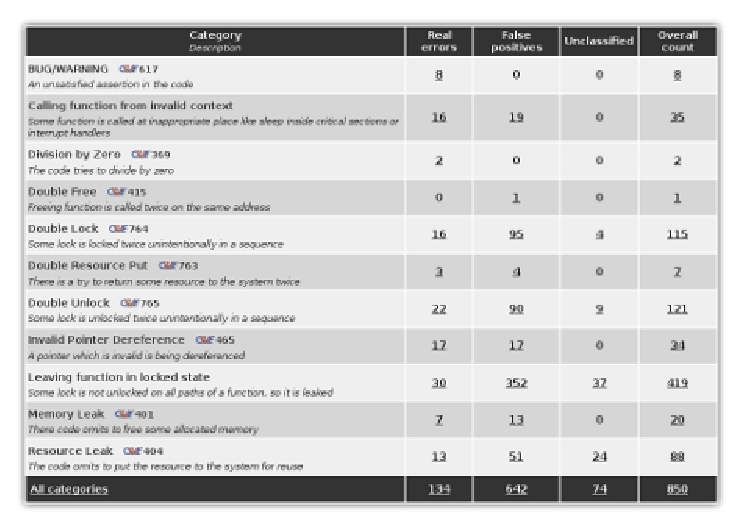
\includegraphics[width=\textwidth]{types}
% \end{center}
% \caption{Error types in the web interface}
% \label{fig:types}
% \end{figure}

% \todo{Zvetsit font ve Fig~\ref{fig:types}, je to necitelny. A budto tu
%   nechat ten obrazek, nebo tabulku. Oboji ne.}

\cdb currently contains only bug-reports produced for the Linux kernel
2.6.28. We have chosen Linux kernel for several reasons: it is a big (20484
files with nearly 9 millions LOC in total), real-life, self-contained, and
open-source project with several public sources of information about
errors. Moreover, the kernel contains many distinct parts (core, hardware
drivers, filesystems, networking etc.) that cover some standard application
areas of program analysis tools.

\subsubsection{Sources of Bug-Reports}

We used three program analysis tools to gather bug-reports for the kernel:
\clang~3~\cite{clang}, \stan 1.2~\cite{stanse}, and one commercial tool
which wanted to stay in anonymity. Note that \clang does not natively detect
locking errors in the Linux kernel. Hence, we slightly modified
\texttt{experimental.unix.PthreadLock} checker just to understand kernel
locking functions. The database also comprises bug-reports from kernel and
Novell bug tracking systems and mailing lists. For that purpose we implemented
our own web crawler. Finally, there are few bug-reports detected manually.

\subsubsection{Linux Kernel Error Types} \label{sec:error_type}

We have analyzed output of available tools applicable to the Linux kernel
and we have decided to focus on the following 11 error types. Nine of these
error types are present in \emph{Common Weakness Enumeration}
(\textsc{CWE})~\cite{cwe} and we provide their CWE identification
numbers. The two remaining error types are specific for the Linux kernel
(they can be seen as a violation of the kernel coding policy) and thus they
are not covered by CWE.

The list of considered error types follows. For each error type we
explicitly describe the program location associated with an error of this
type. This is to evade misinterpretation, because diverse tools can associate
the same error with different program locations. For example, an error
present at an outgoing edge of a function may be associated to the opening
brace of the function, the closing brace, or to the corresponding
\texttt{return} statement.

\begin{description}
\item \textbf{BUG/WARNING} (CWE 617) Developers often inject \emph{assert}s
  to their code, e.g.~to ensure that their function is given a correct input.
  For example, a destroy function of an object \texttt{obj} can contain a
  line \texttt{assert(!obj->active)} to check that the object to be
  destroyed is inactive. An error occurs if a condition of some
  \texttt{assert} is violated.\\
  \emph{Error location:} the line with the violated assertion.
  % where the assertion appears in the code.
\item \textbf{Division by Zero} (CWE 369) The code contains a division
  instruction but the actual value of the divisor
  is zero. \\
  \emph{Error location:} the line with the division.
\item \textbf{Double Lock} (CWE 764) Some lock is locked by a thread twice
  in a row and it leads to an inconsistent lock state. Note that we ignore
  double locks of semaphores as this may be their intentional application.\\
  \emph{Error location:} the line with the second call of lock.
\item \textbf{Double Unlock} (CWE 765) Some lock is unlocked by a thread
  twice in a row and it leads to an
  inconsistent lock state. Again, we ignore double unlocks of semaphores.\\
  \emph{Error location:} the line with the second call of unlock.
\item \textbf{Double Free} (CWE 415) A freeing function is called twice on
  the same address while no reassignment to the passed pointer
  occurred between the two calls. Most allocators can detect this and usually
  kill the program. \\
  \emph{Error location:} the line of the invalid (second) free.
\item \textbf{Memory Leak} (CWE 401)
  Some code omits to free a memory which was allocated previously. \\
  \emph{Error location:} the line with the allocation statement.
\item \textbf{Invalid Pointer Dereference} (CWE 465) The code tries to
  access some memory, but the pointer used is invalid. It may become invalid
  in many ways. For example, the pointer may point to a released memory (known
  as \emph{dangling pointer} or \emph{use after free}) or it can be set to
  NULL (known as \emph{NULL pointer dereference}) or uninitialized. Another
  source of the problem may be accessing an array out of bounds. \\
  \emph{Error location:} the line of the dereference.
\item \textbf{Double Resource Put} (CWE 763) The code requests one copy of a
  resource (e.g.~a structure holding hardware status) from a system, but
  there is more than one attempt to put that resource back to the
  system. Like in this example:
  \begin{lstlisting}[language=C]
struct pci_dev *pdev = pci_get_device(vendor, device, NULL); // get
if (pdev) {
  work_with_pdev(pdev)
  pci_dev_put(pdev);               // first put
}
pci_dev_put(pdev);                 // second (illegal) put of the same
  \end{lstlisting}
  \emph{Error location:} the line of the second put.
\item \textbf{Resource Leak} (CWE 404) The code requests a resource from a
  system, but omits to return that back. For example, the error occurs in
  the previous example if we remove both \texttt{pci\_dev\_put} calls. \\
  \emph{Error location:} the line of the request/get.
% \end{description}
% The following two error types may be only Linux kernel specific. Note that the
% database is not limited to a bounded set of error types. Each project may
% extend this set by arbitrary error types.
% \begin{description}
\item \textbf{Calling Function from Invalid Context} (not in CWE, Linux
  kernel specific) Some function is called at an inappropriate place or within
  an invalid context. This includes calling functions like sleep or wait
  inside spin-lock critical sections or in interrupt handlers. This is
  considered to be an error because results of such a call are undefined: the
  system may become unresponsive or may crash for instance. \\
  \emph{Error location:} the line of the inappropriate call.
\item \textbf{Leaving Function in Locked State} (not in CWE, Linux kernel
  specific) This error type originates from the kernel requirements that a
  process has to release all locks before returning control to userspace.
  This error occurs if a function has an execution path where some lock is
  locked and left locked when leaving the function. It is considered to be
  an error (violation of the kernel coding policy) as such an execution may
  lead to a deadlock on the next invocation of any function wanting to take
  the same lock. \\
  % And yet, this is sometimes reported by tools which analyze a large project
  % per module and start the analysis from some chosen starting functions.  If
  % the lock is locked while leaving these initial
  % functions, the tools generate this report.  \\
  \emph{Error location:} the line of the corresponding \texttt{return}
  statement or closing brace if there is no \texttt{return}.
\end{description}

\begin{table}[tb]
\begin{center}
\small
\setlength{\tabcolsep}{2.5pt}
\begin{tabular}{|l|c|c|c|c|} \hline
\textbf{Error Type} & \textbf{Real Err.} & \textbf{False Pos.} &
	\textbf{Unclassified} & \textbf{Total} \\ \hline
BUG/WARNING & 8 & 0 & 0 & 8 \\
Division by Zero & 2 & 0 & 0 & 2 \\
Double Lock & 16 & 95 & 4 & 115 \\
Double Unlock & 22 & 90 & 9 & 121 \\
Double Free & 0 & 1 & 0 & 1 \\
Memory Leak & 7 & 13 & 0 & 20 \\
Invalid Pointer Dereference & 17 & 17 & 0 & 34 \\ 
\hspace{1em}\cellcolor{black!10}{\scriptsize NULL Pointer Dereference} & 
\cellcolor{black!10}\scriptsize 17 & \cellcolor{black!10}\scriptsize 14 & 
\cellcolor{black!10}\scriptsize 0 & \cellcolor{black!10}\scriptsize 31 \\
\hspace{1em}\cellcolor{black!10}{\scriptsize Use After Free} & 
\cellcolor{black!10}\scriptsize 0 & \cellcolor{black!10}\scriptsize 3 & 
\cellcolor{black!10}\scriptsize 0 & \cellcolor{black!10}\scriptsize 3 \\
Double Resource Put & 3 & 4 & 0 & 7 \\
Resource Leak & 13 & 51 & 24 & 88 \\
Calling function from invalid context & 16 & 19 & 0 & 35 \\
Leaving function in locked state & 30 & 352 & 37 & 419 \\ \hline
\textbf{Overall Count} & 134 & 642 & 74 & 850 \\ \hline
\end{tabular}
\end{center}
\caption{Reports in \cdb.}
\label{tab:reports}
\end{table}

\subsubsection{Bug-Reports in the Database}

Currently the database comprises 850 reports: 134 real errors, 642 false
positives, and 74 entries which are unclassified. Many of the unclassified
entries were added even recently and are about to be classified soon.
Table~\ref{tab:reports} depicts how each kind of bug-reports is represented in
the database. As seen from the table, most of the bug-reports in the database
are related to locking errors. 

% Further, we used our database for comparing kernel subsystems according to
% error occurrence in Table~\ref{tab:stats}. For the presentation purposes we
% excluded subsystems with less than 10 reports. Those were security,
% virtualization, or inter-process-communication subsystems for example. Based
% on the findings of the tools we used, we can see that the highest ratio of
% errors per file is in the sound subsystem and a core code performing memory
% management and maintaining running system. On the other hand we see that the
% tools were very unsuccessful to find real errors in networking subsystem while
% they found relatively many false positives there. The core is the worst
% written code with respect to the tools in this manner. In average, every
% second file contained a false positive.

% What is not in the Table~\ref{tab:stats}, but can be pulled out of \cdb is that
% maximum false positives per file (19) is found in the very core of the kernel
% scheduler in \texttt{kernel/sched.c}. It is followed by the XFS filesystem in
% \texttt{fs/xfs/xfs\_log.c} with 14 hits and directory cache management in
% \texttt{fs/dcache.c} with 12 hits. All of them but two are related to improper
% locking. In most of the cases, the false positives stem from too complex code.
% The tools could not often cope with a conditional call to lock and yet,
% located in a loop.

% \begin{table}[tb]
% \begin{center}
% \setlength{\tabcolsep}{2.5pt}
% \begin{tabular}{|l|c|c|c|c|c|c|} \hline
% \textbf{Subsystem} & \textbf{Files} & \textbf{KLOC} & \textbf{Real Err.} &
% 	\textbf{False Pos.} & \textbf{Errs/file (\%)} & \textbf{FPs/file (\%)} \\ \hline

% Arch        &  354 &  146 &  6 &  15 & 1.69 & 4.24 \\
% Core        &  202 &  166 &  5 & 104 & 2.48 & 51.49 \\ % mm+kern
% Drivers     & 4492 & 4029 & 88 & 205 & 1.96 & 4.56 \\
% Filesystems &  899 &  720 & 16 & 164 & 1.78 & 18.24 \\
% Networking  &  834 &  525 &  5 & 127 & 0.60 & 15.22 \\
% Sound       &  529 &  438 & 13 &  10 & 2.46 & 1.89 \\ \hline

% \textbf{Summary} & 7310 & 6960 & 133 & 625 & 1.82 & 8.55 \\ \hline
% \end{tabular}
% \end{center}
% \caption{Statistics}
% \label{tab:stats}
% \end{table}

%}}}
%{{{ Intended Use of the Database

\subsection{Intended Use of the Database}\label{sec:use}

Typical use of \cdb is tuning and evaluation of a bug-finding program
analysis tool. To evaluate such a tool, one chooses a project (or its part)
from our benchmark suite and run the tool on these source codes.  As the
second step, the sub-database of classified bug-reports corresponding to the
chosen project is downloaded from \cdb.  The installation and local database
usage is described in the \cdb documentation.

The bug-reports produced by the tool are compared to the downloaded data. This
way, one immediately gets a classification (real error/false positive) of all
the reports matched in the database and also information about missed real
errors if there are any. It remains to manually classify the bug-reports
unmatched with the database content. The numbers of produced false positives,
detected and missed real errors can be further statistically processed
according to methodologies of~\cite{begbunch,HW08} which produce several metrics
including accuracy and precision. The missed errors and false positives are
valuable inputs for tuning the tool. 

Finally, the user is kindly asked to insert newly discovered bug-reports with
their classification into the database.  

%}}}
%{{{ Future Plans

\subsection{Conclusion and Future Plans}

We have presented \cdb: the database of classified bug-reports. It is
intended as an open platform for sharing valuable benchmarks for developers
of program analysis tools. The database already contains a large collection
of uniformly described bug-reports produced by various tools on a large
real-life project, namely the Linux kernel 2.6.28.

\medskip
We plan to extend the database in several directions. Namely, we intend to
collect more bug-reports and to support more error types in the Linux kernel
project. For example, we plan to add error types connected to deadlock and
livelock. 
% Note that these errors often need to be represented by more than
% one program point. 
Further, we plan to add other real-life projects. We also plan to extend the
web interface to enable developers of program analysis tools to maintain and
augment the database.

In general, the future of \cdb depends on a feedback from the program analysis
community. At this point, we would like to encourage you to contact us at
\texttt{claburedb@fi.muni.cz} if you have any comments, suggestions (for
example which projects should be added to the database), questions, or
sources of bug-reports for the Linux kernel or other interesting projects. We
would especially welcome people willing to participate on creating and
maintaining the database content for another project.



